\subsection{Kaskadierte Regelsysteme}
    Kaskadierte Regelsysteme eignen sich für SIMO Systeme mit einer schnellen und einer langsamen Teildynamik. Um die olle Bandbreite der schnellen Dynamik auszunützen werden verschiedene Regler für das schnelle und das langsame Teilsystem ausgelegt.
    
    \begin{figure}[H]
        \centering
        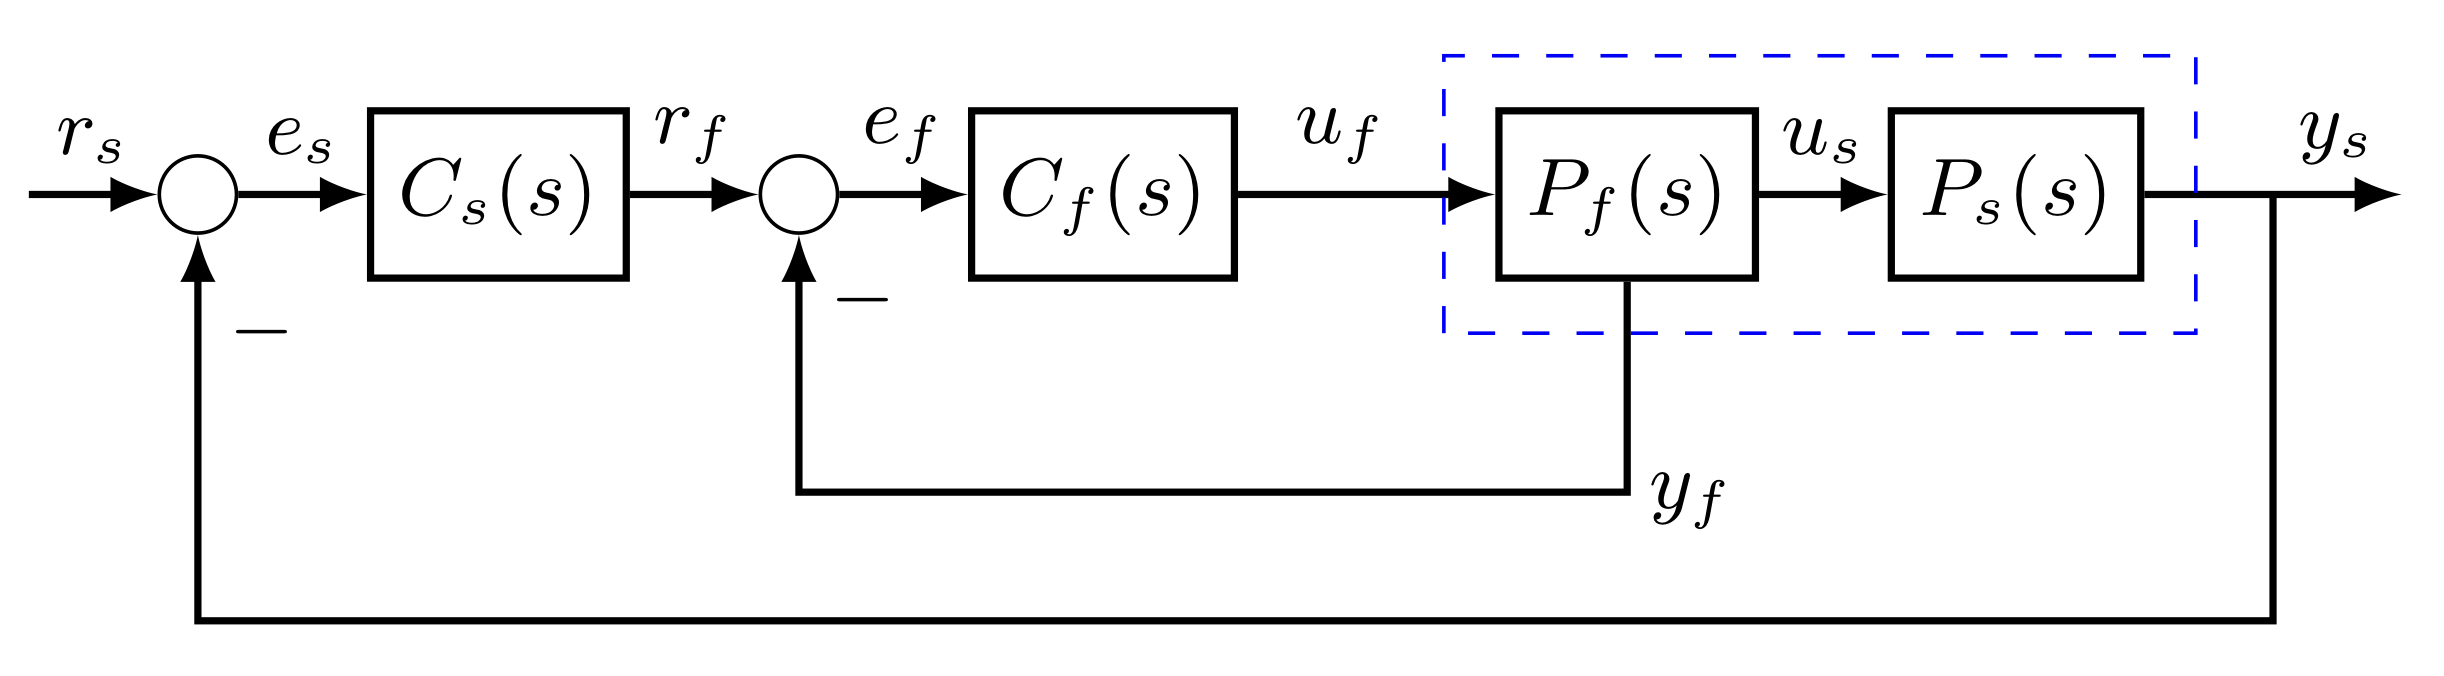
\includegraphics[width = 0.7\linewidth]{images/04/kaskad_sys.jpeg}
        \caption{Kaskadiere Regelstruktur. index $s$ für slow und $f$ für schnell.}
    \end{figure}
    \begin{align*}
        T_{f}(s) &= \frac{L_f(s)}{1 + L_f(s)} = \frac{C_f(s)\cdot P_f(s)}{1 + C_f(s)\cdot P_f(s)}\\
        T_{s}(s) &= \frac{L_s(s)}{1 + L_s(s)} = \frac{C_s(s)\cdot T_{f}(s)\cdot P_s(s)}{1 + C_s(s)\cdot T_f(s) \cdot P_s(s)}
    \end{align*}
    Um die Bandbreite des schnellen Systems auszunutzen wird für $C_f(s)$ oftmals kein Integrator verwendet (verlangsamt). Der Integrator wird in $C_s(s)$ integriert um einen statischen Nachlauffehler zu eliminieren.
    
    \subsubsection{Bsp}
        Masse auf einem Wagen mit einem Feder Dämpfer System an der Wand befestigt.
        \begin{figure}[H]
            \centering
            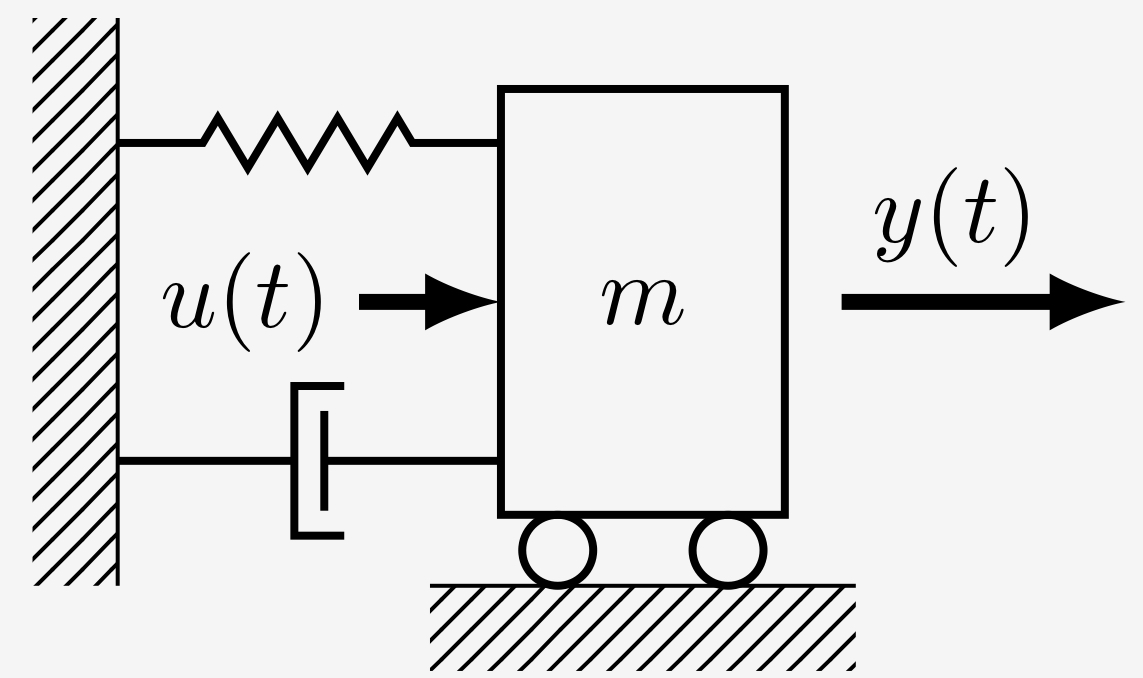
\includegraphics[width = 0.25\linewidth]{images/04/kask_bsp.jpeg}
        \end{figure}
        Man will die Position regeln. Man stellt jedoch fest, dass $u(t)$ direkt auf $v(t)$ wirkt und nur auf indirekt die Position $x(t)$.
        \begin{align*}
            u\rightarrow v: \qquad &P_f(s) = \frac{s}{s^2+s+1}\\
            v\rightarrow x: \qquad &P_s(s) = \frac{1}{s}\\
            u\rightarrow x: \qquad &P(s) = \frac{1}{s^2+s+1}
        \end{align*}
        Auch stellt man fest, dass die Pole von $P_f(s)$ $\pi(P_f(s) = -\frac{1}{2}\pm j\frac{\sqrt{3}}{2}$ einen negativeren Realteil haben als der Pol von $P_s(s)$. \textbf{Pole mit grösserem negativen Realteil klingen schneller ab.}
        
        $P_f$ ist definitiv schneller als $P_s$. Obwohl $\pi(P) =\pi(P_f)$ wird $P_f$ schneller sein, da das System $P$ durch den zusätzlichen offenen Integrator einen grösseren Phasenverlust hat.
        
        Es bietet sich an für $C_f$ einen P-Regler und für $C_s$ einen PI-Regler zu verwenden.